\section{MSLList  Class Template Reference}
\label{classMSLList}\index{MSLList@{MSLList}}
{\tt \#include $<$msllist.h$>$}

Inheritance diagram for MSLList::\begin{figure}[H]
\begin{center}
\leavevmode
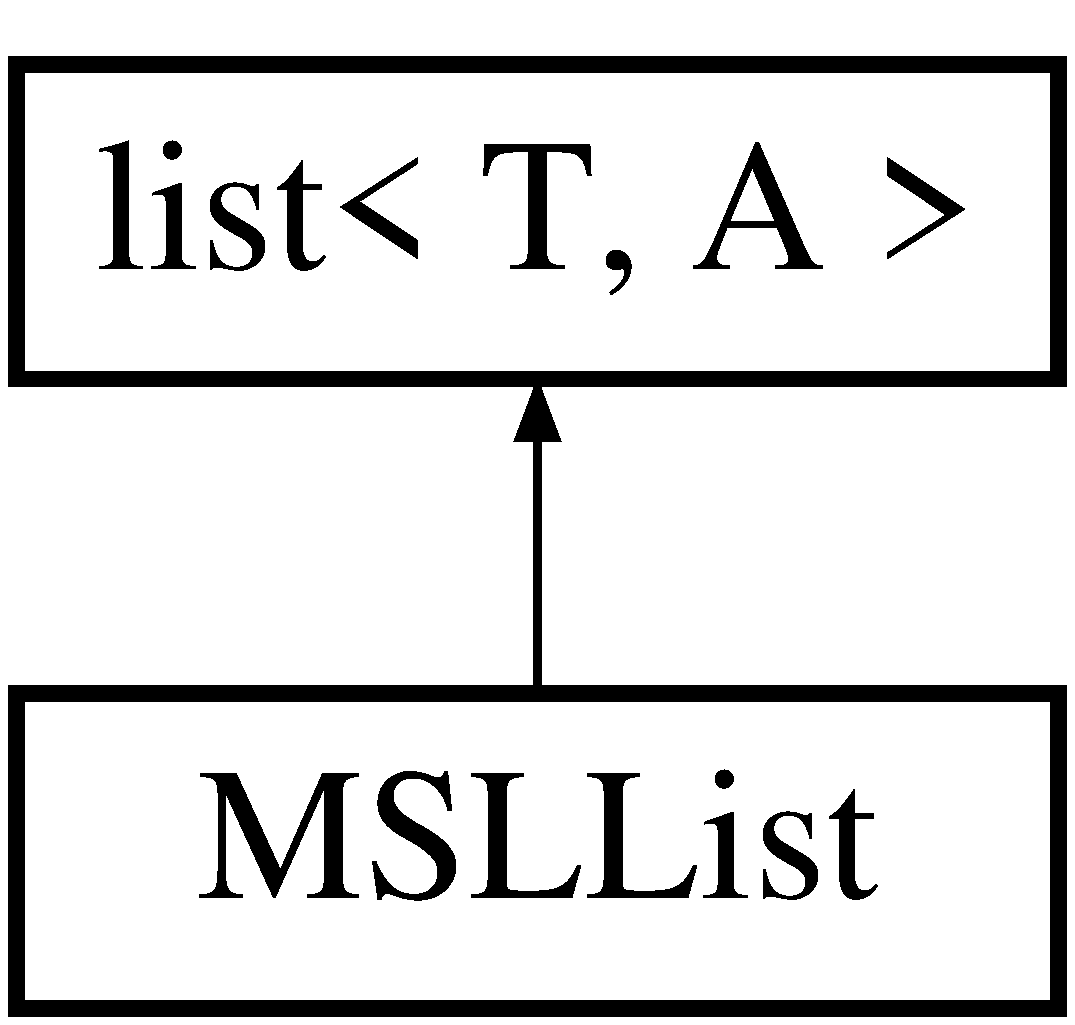
\includegraphics[height=2cm]{classMSLList}
\end{center}
\end{figure}
\subsubsection*{template$<$class T, class A = allocator$<$T$>$$>$  class MSLList}



\subsection{Friends And Related Function Documentation}
\index{MSLList@{MSLList}!operator<<@{operator$<$$<$}}
\index{operator<<@{operator$<$$<$}!MSLList@{MSLList}}
\subsubsection{\setlength{\rightskip}{0pt plus 5cm}template$<$class T, class A = allocator$<$T$>$$>$ ostream \& operator$<$$<$ (ostream \& {\em out}, const MSLList$<$ T $>$ \& {\em L})\hspace{0.3cm}{\tt  [friend]}}\label{classMSLList_l0}


\index{MSLList@{MSLList}!operator>>@{operator$>$$>$}}
\index{operator>>@{operator$>$$>$}!MSLList@{MSLList}}
\subsubsection{\setlength{\rightskip}{0pt plus 5cm}template$<$class T, class A = allocator$<$T$>$$>$ istream \& operator$>$$>$ (istream \& {\em in}, MSLList$<$ T $>$ \& {\em L})\hspace{0.3cm}{\tt  [friend]}}\label{classMSLList_l1}




The documentation for this class was generated from the following file:\begin{CompactItemize}
\item 
{\bf msllist.h}\end{CompactItemize}
